\documentclass{beamer}

\usepackage[latin10]{inputenc}
\usepackage{color}
\usepackage{ae}
\usepackage{graphicx}
\usepackage{algorithmic}
%\usepackage{epstopdf}
%\usepackage[pdftex]{graphicx}

\usepackage{multimedia}
\usepackage{multicol}
\usepackage{hyperref}
\usepackage{verbatim}
\usepackage{alltt}
\usepackage{listings}
\usepackage{mathpartir}

\definecolor{darkblue}{rgb}{0,0,0.5}

\mode<presentation>
{
  \usetheme{Warsaw} %
  \usecolortheme{orchid}
  \usefonttheme[onlysmall]{structurebold}
  \beamertemplateballitem
}


\setbeamercovered{dynamic}
\setbeamercovered{transparent}

\title{{\bf Lazart: a symbolic approach for evaluating the robustness of secured codes 
             against control flow fault injections}}
\author{M. L. Potet \and \underline{L. Mounier} \and M. Puys \and L. Dureuil}
\institute{{\bf\large VERIMAG} \\ ~ \\ {\bf\large University of Grenoble Alpes, France}}
%\author{{\bf VERIMAG} \\ University of Grenoble}
\date{ICST 2014 - Cleveland } 

\useheadtemplate{}

\definecolor{grey}{rgb}{0.7,0.7,0.7}
\definecolor{gg}{rgb}{0.85,0.85,0.85}
\definecolor{bb}{rgb}{0.4,0.4,0.4}
%Define colors
\definecolor{blue2}{rgb}{0.3,0.7,1}
\definecolor{blue3}{rgb}{0.4,0.75,1}
\definecolor{blue4}{rgb}{0.55,0.8,1}
\definecolor{blue5}{rgb}{0.7,0.85,1}

%define colors by uses
\definecolor{simcolor}{cmyk}{0.683, 0.482, 0, 0.145} % couleur du simulateur
\definecolor{modcolor}{cmyk}{0.119, 0.547, 0, 0.376} % couleur du modele
\definecolor{gencolor}{cmyk}{0, 0.75, 1, 0.2} % couleur du generateur
\definecolor{filecolor}{cmyk}{0, 0.109, 0.271, 0.031} % couleur des entrees/sorties
\definecolor{gramcolor}{cmyk}{0, 0.4, 1, 0} % couleur du module de grammaire
\definecolor{chipcolor}{cmyk}{0, 0.153, 1, 0} % couleur de la chip d'une càp
\definecolor{attackcolor}{cmyk}{0, 0.2, 1, 0} % couleur des attaques

\definecolor{cpucolor}{cmyk}{0,0.492,0.41,0.522} % couleur du processeur
\definecolor{cocolor}{cmyk}{0.5,1,0,0.2} % couleur des coprocesseurs
\definecolor{memcolor}{cmyk}{0.742,0,0.05,0.529} % couleur de la mémoire
\definecolor{buscolor}{cmyk}{0.555,0,0.486,0.427} % couleur du bus de données
\definecolor{circolor}{cmyk}{0,0,0,0.4} % couleur du fond de circuit

\definecolor{trigcolorleft}{HTML}{7ACC29}
\definecolor{trigcolorright}{HTML}{19D1FF}
\definecolor{trigcolorbottom}{HTML}{336680}

\usepackage{tikz}
\newsavebox\chip
\sbox{\chip}{

\begin{tikzpicture}[remember picture,
scale=0.07,
% define styles here
chiplayout/.style={rectangle, draw, fill=chipcolor, rounded corners}
]
\draw[chiplayout] (0, 0) rectangle (9,8);
\draw (3, 0) -- (3, 8);
\draw (3, 2) -- (0, 2);
\draw (3, 4) -- (0, 4);
\draw (3, 6) -- (0, 6);

\draw (6, 0) -- (6, 6);
\draw (6, 2) -- (9, 2);
\draw (6, 4) -- (9, 4);
\draw (6, 6) -- (9, 6);
\end{tikzpicture}
}

\tikzset{middlearrow/.style={
        decoration={markings,
            mark= at position 0.5 with {\arrow{#1}} ,
        },
        postaction={decorate}
    }
}




%\usepackage{pgfgantt}
\usetikzlibrary{mindmap,backgrounds}
\usetikzlibrary{shapes}
\usetikzlibrary{shapes.symbols}
\usetikzlibrary{decorations.pathreplacing}
\usetikzlibrary{decorations.markings}

% tikz block styles
\tikzstyle{decision} =  [diamond, draw, fill=blue!20,
text width=5.5em, text badly centered, node distance=3.2cm, inner
sep=0pt]
\tikzstyle{block} = [rectangle, draw, fill=blue!20,
text width=7.0em, text centered, node distance=3.2cm, rounded corners, minimum height=3em]
%\tikzstyle{line} = [draw, -latex']
\tikzstyle{line} = [draw]
\tikzstyle{cloud} = [draw, ellipse, fill=red!20, node distance=3cm, 
minimum height=2em]


% attaques
\def\attaqueasma{\only<1,3,4>{\#00}\only<2>{\colorbox{attackcolor}{\#2a}}}
\def\attaqueasmb{\only<1,2,4>{\#04}\only<3>{\colorbox{attackcolor}{\#ff}}}
\def\attaqueasmc{\only<1,2,3>{\textcolor{green!40!black}{JNC} \textcolor{blue}{DO}}\only<4>{\colorbox{attackcolor}{NOP NOP}}}

\def\attaqueca{\only<1,3,4>{0}\only<2>{\colorbox{attackcolor}{42}}}
\def\attaquecb{\only<1,2,4>{4}\only<3>{\colorbox{attackcolor}{-1}}}
\def\attaquecca{\only<1,2,3>{\itshape\color{purple!40!black}// main loop}
\only<4>{\colorbox{attackcolor}{goto ATTACK;}}}


\def\attaqueccb{\only<1,2,3>{\itshape\color{purple!40!black}// The
comparison is successful}
\only<4>{\colorbox{attackcolor}{ATTACK:}}}

\def\firstcircle{(0,0) circle (2.4cm)}

\def\secondcircle{(45:1.8cm) circle (2.4cm)}
\def\thirdcircle{(0:2.4cm) circle (2.4cm)}


\usefoottemplate{\vbox{%
\hbox{
%\tinycolouredline{black}%
%{\color{white}\textbf{\insertshortauthor}}%
%\tinycolouredline{darkblue}
%{\color{white}\textbf{\insertframenumber/\inserttotalframenumber}} 
%}
\tinycolouredline{structure}%
{\color{white}\textbf{\insertshorttitle}\hfill \textbf{\insertframenumber/\inserttotalframenumber}}%
}
}}


\lstdefinestyle{customc}{
  belowcaptionskip=1\baselineskip,
  breaklines=true,
  frame=L,
  xleftmargin=\parindent,
  language=C,
  showstringspaces=false,
  basicstyle=\scriptsize\ttfamily,
  keywordstyle=\bfseries\color{green!40!black},
  %commentstyle=\itshape\color{purple!40!black},
  commentstyle=\itshape\color{red},
  identifierstyle=\color{blue},
  stringstyle=\color{orange},
}

\lstdefinestyle{customasm}{
  belowcaptionskip=1\baselineskip,
  frame=L,
  xleftmargin=\parindent,
  language=[x86masm]Assembler,
  basicstyle=\tiny\ttfamily,
  commentstyle=\itshape\color{purple!40!black},
  morecomment=[l]{//},
  morekeywords={SUBB},
}

\lstset{ numbers=left, tabsize=3, frame=single, numberstyle=\ttfamily,
basicstyle=\footnotesize, escapechar=@,style=customc,
           captionpos=b, % sets the caption position to bottom
               extendedchars=false, % for babel compatibility
}


\newcommand{\fleche}[1]{\;\stackrel{\mbox{\scriptsize {#1}}}{\longrightarrow}\;}
\newcommand{\IGNORE}[1]{}

\newcommand{\reil}{{\sc Reil}}
\newcommand{\noval}{\mbox{None}}
\newcommand{\initesp}{\mbox{InitEsp}}
\newcommand{\anyval}{\mbox{Any}}
\newcommand{\emptyval}{\mbox{Empty}}
\newcommand{\ZZ}{\mathbb{Z}}

\newcommand{\texte}[1]{\;\mbox{#1}\;}
\newcommand{\AVOIR}[1]{\fbox{#1}}

\begin{document}

\begin{frame}
\titlepage

\noindent 
\includegraphics[height=1.5cm]{logoverimag.jpg} 
\end{frame}

\section{Context and Motivation}

%\begin{frame}
%    \frametitle{Outline}
%    \tableofcontents[]
%\end{frame}

\begin{frame} \frametitle{Context: smart card certification}
\vfill
% Composants sécurisés = cartes à puce : utilisées partout
% PEUVENT ÊTRE ATTAQUEES ! Par un voleur, l'utilisateur, etc...
% Sont protégées et leur sécurité est évaluée avant leur mise sur le marché
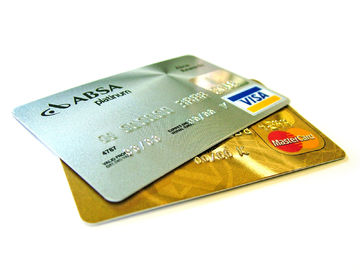
\includegraphics[height=1cm]{sm1.jpg} 
\vfill
\begin{block}{Smart cards}
\begin{itemize}
\item Pervasive : bank, health, phones, \ldots (7 billions sold in 2012) 
\vfill
\item Contain sensible data and applications 
		\alert{{\bf $\Rightarrow$ can be attacked!}}
\end{itemize}
\end{block}
\vfill
\begin{block}{Smart card security}
\begin{itemize}
	\item Protections mechanisms added by manufacturers 
	\item Well-defined \alert{certification process}, prior to commercialization:
	\begin{itemize}
		\item Security functional test
		\item \alert{Penetration test} 
	\end{itemize}
\end{itemize}
\end{block}
\begin{block}{Certification procedures include}
	\begin{itemize}
	\item Physical testing on the device (black box)
	\item \alert{Code review and/or code analysis (white box)}
	\end{itemize}
\end{block}
\vfill
\end{frame}

%\IGNORE{
%\begin{frame} \frametitle{A typical certification process}
%\vfill
%\begin{figure}
%\begin{tikzpicture}[scale=0.60,every node/.style={transform shape}] 
%    % Place nodes
%    \node [decision] (oktestsw) {Are tests OK?};
%    \node [block, left of=oktestsw] (testsw) {Try to forecast vulnerabilities};
%    \node [block, left of=testsw] (code) {Develop secure application};
%    \node [block, right of=oktestsw] (eval) {Evaluate conformity and vulnerabilities};
%    \node [decision, right of=eval] (okeval) {Is evaluation OK?};
%    \node [block, right of=okeval] (cert) {Emit certificate};
%    %actors
%    \node [cloud, below of=code] (dev) {Developer};
%    \node [cloud, below of=eval] (cesti) {ITSEF (CESTI)};
%    \node [cloud, below of=cert] (anssi) {ANSSI};
%
%        %conditions
%    % Draw edges
%    %actors -- actions
%    \path [line, dashed] (dev) -- (code);
%    \path [line, dashed] (dev) -- (testsw);
%    \path [line, dashed] (cesti) -- (eval);
%    \path [line, dashed] (anssi) -- (cert);
%    % actions -- next_actions
%    \path [line] (code) -- (testsw);
%    % actions -- decisions
%    \path [line] (eval) -- (okeval);
%    \path [line] (testsw) -- (oktestsw);
%    % decisions -- actions
%    \path [line] (oktestsw) -- +(0, 2) -| node[near start, above] {no}(code);
%    \path [line] (oktestsw) -- node[above] {yes}(eval);
%    \path [line] (okeval) -- +(0, 3) -| node[near start, above] {no}(code);
%    \path [line] (okeval) -- node[above] {yes}(cert);
%\end{tikzpicture}
%\end{figure}
%\vfill
%\pause
%$\rightarrow$ Evaluation performed according to the \alert{Common Criteria}
%\begin{itemize}
%	\item black box: physical testing on the device
%	\item white box: code review and/or code analysis 
%\end{itemize}
%\vfill
%\end{frame}
%}
%
%
%\begin{frame} \frametitle{Fault injection based attacks}
%% L'injection de faute est 1 attaque réalisée physiquement qui change l'exec
%\vfill
%$\bullet$ physical attack performed at runtime \\
%	$\quad$ $\leadsto$
%\textbf{change the data read} or  \textbf{modify the executed code} \\
%$\bullet$ several techniques: \\ $\quad$ laser/electromagnetic perturbation, clock acceleration \dots
%%A model for what happens:
%    \begin{figure}
%    \begin{tikzpicture}[remember picture,
%    scale=0.80,
%    % define styles here
%    every node/.style={transform shape}
%    ]
%    \draw[rounded corners] (0, 0) rectangle (5, 3);
%
%    \node (chip) at (0.7,2) { \usebox\chip };
%    \draw[fill=circolor] (1.4, 0.4) rectangle (4.6, 2.6);
%    \node[fill=cpucolor] (CPU) at (2.0, 1.5) [draw, thick, minimum width=1.0cm,
%    minimum height=2.0cm, font=\small] {\textbf{CPU}};
%    \node[fill=memcolor] (Mem) at (4.0, 2.25) [draw, thick, minimum width=1.0cm,
%    minimum height=0.5cm, font=\small] {\textbf{Mem}};
%    %\draw[fill=buscolor] (2.5, 1.3) rectangle (3.5, 1.7) node[font=\tiny, midway]{Bus};
%    \draw[middlearrow={<}, very thick] (CPU) -- (4.0, 1.5) -- (Mem);
%    \draw[color=attackcolor] (3.25, 1.80) -- (3.05, 1.60) --
%    (3.25, 1.40) -- (3.05, 1.20)
%        node[color=attackcolor, midway, below]{\scriptsize{attack}};
%    \node[font=\scriptsize] (valmem) at (4.3, 1.8) {0x3a};
%    \node[font=\scriptsize, color=red] (valcpu) at (2.8, 1.35) {0x42};
%    \end{tikzpicture}
%    \end{figure}
%\vfill
%% Au niveau binaire ça donne :
%\vfill
%\begin{table}
%\centering
%%% init
%\only<1>{
%\begin{tabular*}{0.99\linewidth}{|c @{\extracolsep{\fill}}||c|c|c|}
%\hline
%Instruction             & \multicolumn{3}{c|}{LD R0 M[23] ; Loads M[23]=0x72 in R0} \\
%\hline
%Memory access number    & 1         & 2         & 3 \\
%Address                 & 0xEE1223  & 0xEE1224  & 0x23 \\
%Value                   & 0x87      & 0x23      & 0x72 \\
%\hline
%\end{tabular*}
%}
%\only<2>{
%%% perturbation n°1
%\begin{tabular*}{0.99\linewidth}{|c @{\extracolsep{\fill}}||c|c|c|}
%\hline
%Instruction             & \multicolumn{3}{c|}{LD R0 23 ; Loads
%immediate 0x23 in R0} \\
%\hline
%Memory access number    & 1         & 2         & 3 \\
%Address                 & 0xEE1223  & 0xEE1224  & Discarded \\
%Value                   & \textbf{\textcolor{red}{0x42}}
%& 0x23      & Discarded \\
%\hline
%\end{tabular*}
%}
%\only<3>{
%%% perturbation n°2
%\begin{tabular*}{0.99\linewidth}{|c @{\extracolsep{\fill}}||c|c|c|}
%\hline
%Instruction             & \multicolumn{3}{c|}{LD R0 M[42] ; Loads
%M[42]=0x66 in R0} \\
%\hline
%Memory access number    & 1         & 2         & 3 \\
%Address                 & 0xEE1223  & 0xEE1224  & 0x42 \\
%Value                   & 0x87      & \textbf{\textcolor{red}{0x42}}      & 0x66 \\
%\hline
%\end{tabular*}
%}
%\only<4>{
%%% perturbation n°3
%\begin{tabular*}{0.99\linewidth}{|c @{\extracolsep{\fill}}||c|c|c|}
%\hline
%Instruction             & \multicolumn{3}{c|}{LD R0 M[23] ; Loads 0x42 in R0} \\
%\hline
%Memory access number    & 1         & 2         & 3 \\
%Address                 & 0xEE1223  & 0xEE1224  & 0x23 \\
%Value                   & 0x87      & 0x23      & \textbf{\textcolor{red}{0x42}} \\
%\hline
%\end{tabular*}
%}
%\only<1>{\caption{Initial instruction}}
%\only<2>{\caption{Opcode perturbation}}
%\only<3>{\caption{Operand perturbation}}
%\only<4>{\caption{Data perturbation}}
%\end{table}
%\vfill
%\end{frame}

\begin{frame}[fragile] \frametitle{Effects of fault injection at the source level}
% Au niveau source ça peut se traduire par :
\begin{columns}[t]
\begin{column}{0.50\textwidth}
\begin{lstlisting}[
  basicstyle=\footnotesize\ttfamily,
]
int verify(char buffer[4]) 
{
  int i;
  for(i = 0; i < 4; i++)
    if(buffer[i] != pin[i]) {
      authenticated = 0;
      goto FAILURE;
    }
  authenticated = 1;
  return EXIT_SUCCESS;
  FAILURE : return EXIT_FAILURE;
}
\end{lstlisting}
\end{column}
\begin{column}{0.48\textwidth}
\begin{lstlisting}[style=customasm,
%\begin{lstlisting}[language={[x86masm]Assembler},
  basicstyle=\footnotesize\ttfamily,
]
MOV R3, #01h 
MOV R0, #00h
WHILE: MOV A, R0
SUBB A, #04h
JZ END // exit loop
DO:
MOV R2, [buffer+i] 
MOV A, [pin+i] 
SUBB A, R2 
JZ SUCCESS 
MOV R3, #00h
JMP END

SUCCESS: INC R0
JMP WHILE

END: MOV authenticated, R3
RET
\end{lstlisting}

\end{column}
\end{columns}
\end{frame}

%\begin{frame} \frametitle{Code-level protections against fault injections}
%\vfill
%% Problème : la combinatoire des injection
%\begin{block}
%{State of the art in fault injection attacks}
%\begin{itemize}
%\item volatile faults, occuring at run-time ($\neq$ code modification)
%\item multiple spatial and/or temporal faults (up to 2)
%\end{itemize}
%\begin{center}
%\fbox{
%	\alert{$\rightarrow$  
%		impossible to check all fault combinations in practice \dots}
%}
%\end{center}
%\end{block}
%\vfill
%\pause
%\begin{block}
%{Code-level counter-measures}
%\begin{itemize}
%\item instruction counters, check call/exit procedure consistency
%\item duplicated evaluation of conditional expressions
%\item duplicated procedure execution
%\item split/replicate information in several memory locations 
%\item etc.
%\end{itemize}
%\begin{center}
%\fbox{\alert{Are these counter-measures useful ? sufficient ?}}
%\end{center}
%\end{block}
%\vfill
%\end{frame}
%
%\begin{frame}[fragile] \frametitle{Counter-measure examples}
%\begin{lstlisting}[
%  basicstyle=\scriptsize\ttfamily,
%  commentstyle=\color{red}
%]
%int stepCounter = INITIAL_VALUE ; // Instruction counter
%
%int verify(char buffer[4]) {
%  int i;
%  for(i = 0; i < 4; i++) {
%    if(buffer[i] == pin[i]) {
%       if(buffer[i] != pin[i]) {  // Duplicated test
%          authenticated = 0;
%          goto FAILURE;
%       } else {
%          authenticated = 0;
%          goto FAILURE;
%       } ;
%       stepCounter ++ ; // Increment the inst. counter
%    } ;
%  if (stepCounter == INITIAL_VALUE + 4) { 
%     authenticated = 1;
%     return EXIT_SUCCESS; // Each pin byte double checked
%  } else {
%     authenticated = 0 ;
%     goto FAILURE ;
%  } ;
%FAILURE : return EXIT_FAILURE;  // Card is lost ...
%}
%\end{lstlisting}
%
%\end{frame}


%\begin{frame} \frametitle{Work Objective: Developer/Auditor point of view}
%\vfill
%\begin{block}
%{$\rightarrow$ Assist the robustness evaluation against fault injection}
%\vfill
%\begin{itemize}
%\item White box evaluation as a source-level code analysis
%\item Handle state-of-the-art attacks: multiple volatile faults  
%\end{itemize}
%\end{block}
%\vfill
%$\rightarrow$ To be completed with more specific analysis, simulation, physical testing, etc.
%\vfill
%\end{frame}

\begin{frame} \frametitle{Security Property and Fault Model}
\vfill
\begin{block}{Security Property}
\begin{center}
$\hookrightarrow$ \alert{Enforce} or \alert{prevent} the execution of specific instruction(s).
\alert{$\Rightarrow$ Attack Objective = set of basic blocks (not) to be reached} 
\end{center}
\end{block}
\vfill
\begin{block}
{Objectives of the analysis:} 
\begin{itemize}
\item \alert{Predict} (or \alert{prove the absence of}) possible attacks,
		for a given fault model
\item \alert{Locate} the ``dangerous spots'' in the code 
\item \alert{Evaluate} the relevance of existing counter-measures 
\end{itemize}
\end{block}
\vfill
\begin{block}{Fault Model - Multiple faults}
Volatile control structure \alert{test inversion} (e.g., {\tt if}, {\tt while}, etc.) \\
$\hookrightarrow$ Encompass multiple binary-level attacks, e.g.,
\begin{itemize} 
\item NOP injection, modify flag or register value, \dots
\end{itemize} 
\end{block}
\vfill
\end{frame}









\section{The Lazart Approach}


%\begin{frame}
%    \frametitle{Outline}
%    \tableofcontents[]
%\end{frame}


\newcommand{\Green}{\colorbox{green}{Green}}
\newcommand{\Red}{\colorbox{red}{Red}}
\newcommand{\Yellow}{\colorbox{yellow}{Yellow}}
\newcommand{\Orange}{\colorbox{orange}{Orange}}

%\begin{frame} \frametitle{The Lazart approach}
%\vfill
%\begin{block} {Inputs}
%\begin{itemize}
%\item the source (LLVM) code of the target application
%\item an attack objective (from the attacker point of view)
%\item a fault model 
%	%control-flow alteration by condition inversion
%\end{itemize}
%\end{block}
%\vfill
%\pause
%\begin{block}{Processing steps}
%\begin{enumerate}
% \item reachability analysis on the control-flow graph \\
%	$\rightarrow$ identify vulnerable code locations 
% \item (high-order) mutant generation  \\
%	$\rightarrow$ 1 mutant encoding all possible fault combinations
%\item  symbolic test case generation \\ 
%	\begin{itemize}
%	\item exercise ``all possible'' executions (w.r.t a coverage criterion) \\
%	\item  1 execution = inputs + potential faults 
%	\end{itemize}
%\begin{center}
%	\alert{{\bf $\Rightarrow$ find the executions satisfying the attack objective \dots}}
%\end{center}
%%Choix de la représentation intermédiaire LLVM : bon niveau de granularité pour les mutants + un outil de génération de cas de tests symbolique (KLEE)
%\end{enumerate}
%\end{block}
%\vfill
%\end{frame}


%\begin{frame}[fragile]{Example: a (non-robust) PIN verification procedure} 
%\vfill
%\begin{footnotesize}
%\begin{lstlisting}
%#define maxTries 3
%typedef unsigned char BYTE;
%BYTE triesLeft = maxTries;
%BYTE authenticated = 0;
%BYTE pin[4] = {(char)1, (char)2, (char)3, (char)4};
%BYTE Verify(char buffer[4]) {
%        BYTE i;
%        // No comparison if PIN is blocked
%        if(triesLeft <= 0) goto FAILURE;
%        // Main Comparison
%        for(i = 0; i < 4; i++)       
%                if(buffer[i] != pin[i]) {
%                    triesLeft--;
%                    authenticated = 0;
%                    goto FAILURE;
%                }
%        // Comparison is successful
%        triesLeft = maxTries;
%        authenticated = 1;   // bloc bb5: TO BE REACHED !
%        return EXIT_SUCCESS;
%    FAILURE : return EXIT_FAILURE; // NOT TO BE REACHED !
%}
%\end{lstlisting}
%\end{footnotesize}
%\vfill
%\end{frame}
%
%\begin{frame} \frametitle{Step 1: Control-Flow-Graph reachability analysis}
%\vfill
%CFG decision nodes influencing the attack objective ${\cal O}$?  \\
%(assuming ${\cal O}$ is a set of nodes ``to be reached'')
%\pause
%\vfill
%\begin{block}{$\rightarrow$ Computes four subsets of the CFG nodes:}
%\vfill
%\begin{itemize}
%\item \Green\ nodes: eventually lead to ${\cal O}$ \\
% $\hspace*{.5cm}\mbox{{\em lfp} of}~Green=\{{\cal O}\} \cup\ (\{ n : Sons(n) \subseteq\ Green\}\backslash Leaf)$
%
%\vfill\pause
%\item \Red\ nodes: cannot lead to ${\cal O}$ \\
% $\hspace*{.5cm}\mbox{{\em gfp} of}~Red= \{n :  Sons(n) \subseteq  Red)\} \backslash \{{\cal O}\}$
%
%\vfill\pause
%\item \Yellow\ nodes: may lead to ${\cal O}$ \\
%$\hspace*{.5cm}Yellow= N \backslash (Green \cup Red)$
%
%\vfill\pause
%\item \Orange\ nodes: Yellow nodes with a Red son \\
%$\hspace*{.5cm}Orange= \{n :  n \in Yellow \land\ (Sons(n) \cap  Red \not= \emptyset)\} $
%\end{itemize}
%\end{block}
%%popint fixes et CTL
%\vfill\pause
%(Invert \Green and \Red if ${\cal O}$ is a set of nodes ``not to be reached'')
%\vfill
%\end{frame}

\begin{frame} \frametitle{The complete tool chain}
\vfill
\includegraphics[width=\textwidth]{fig_lazard_implem.pdf} 
\vfill
\end{frame}

\begin{frame} \frametitle{Step 1: CFG-coloring}
\vfill
\begin{columns}[t]
\begin{column}{0.40\textwidth}
\includegraphics[height=8cm]{simpleverify.pdf} 
\end{column}
\begin{column}{0.40\textwidth}
\includegraphics[height=8cm]{simplebb5color.pdf} 
\end{column}
\end{columns}
\vfill
\end{frame}

%\begin{frame} \frametitle{Step 2: Mutant Generation}
%\vfill
%$\rightarrow$ Introduce a (potential) attack at each \alert{relevant} decision node
%\vfill \pause
%\begin{block}{Mutation strategy}
%\begin{table}[htb]
%\begin{center}
%\begin{scriptsize}
%\begin{tabular}{|l|c|}
%\hline
%{\bf CFG decision node} & {\bf Mutation} \\
%\hline
%\Green & no mutation \\
%\hline
%\Orange & \alert{{\bf enforce}} reachability of the non \Red son \\
%\hline
%\Red & unreachable  \\
%\hline
%\Yellow  & \alert{{\bf possibly invert}} the test  \\
%with a \Green son~ & to reach the \Green son \\
%\hline
%\Yellow  & \alert{{\bf possibly invert}} the test   from one son \\
%with two \Yellow sons~ & to the other, and vice-versa  \\
%\hline
%\end{tabular}
%\end{scriptsize}
%\end{center}
%\end{table}
%\end{block}
%\vfill \pause
%\begin{block}{High-order mutant}
%\begin{itemize}
%	\item each optionnal mutation $i$ guarded by an extra boolean ${\tt\footnotesize activ}_i$
%	\item computes the effective total number of {\tt faults} introduced
%\end{itemize}
%\end{block}
%\vfill
%\end{frame}



\begin{frame}[fragile]{Step 2: Mutation operators}
\vfill
\begin{center}
{\bf\large Example: mandatory mutation operator}
\end{center}
\vspace{-1em}
\begin{columns}[t]
\begin{column}{0.45\textwidth}
\includegraphics[height=3cm]{mut1.pdf} 
\end{column}
\begin{column}{0.45\textwidth}
\includegraphics[height=4cm]{mut2result.pdf} 
\end{column}
\end{columns}
\vfill
\begin{block}{More complex mutation operators}
\begin{itemize}
	\item Using only mandatory mutations guarantees adversary to reach the objective.
	\item More mutation operators describing optional faults the adversary can use to optimize his attack path.
    \item Guarded by boolean values named {\tt activ\_i}.
\end{itemize}
\end{block}
\vfill
\end{frame}

%\IGNORE{
%\begin{frame}[fragile]{Mutant produced for the {\tt Verify} example}
%\vfill
%At the source level:
%\vfill
%\begin{scriptsize}
%\begin{lstlisting}
%BYTE Verify(BYTE buffer[4]) {
%   int i=0; fault=0;
%// Mandatory mutation on entry: FAILURE/bb
%   if (triesLeft <= 0) fault++;  
%// Optional mutation on bb4: bb1/bb5
%   while (i < 4) {
%      int activbb5 ;
%      klee_make_symbolic(&activbb5,sizeof(int),"activbb5");
%      if(activbb5==1) {fault++; break ;}
%      // body execution
%// Mandatory mutation on bb1: bb2/bb3
%         if(buffer[i] != pin[i]) fault++;
%         i++ ;
%    }
%// Comparison is successful: this block is always reached.
%   triesLeft = maxTries;
%   authenticated = 1;
%   return EXIT_SUCCESS; 
%}
%\end{lstlisting}
%\end{scriptsize}
%\vfill
%$\rightarrow$ in practice the mutant is produced at the LLVM level \dots
%\vfill
%\end{frame}
%}


\begin{frame} \frametitle{Step 3: Symbolic execution}
\vfill
$\hookrightarrow$ Produce ``all possible'' mutant executions \dots
\vfill
\begin{block}{Symbolic values}
\begin{itemize}
	\item Attack activation guards {\tt activ\_i}.
	\item Security-relevant external inputs (e.g., PIN input values).
\end{itemize}
\end{block}
\vfill
\begin{block}{Assertions}
\begin{itemize}
	\item Inputs constraints (e.g., the entered PIN is incorrect).
	\item Maximal fault number (e.g., {\tt fault <= 2}).
\end{itemize}
\end{block}
\vfill
\begin{block}{Coverage criteria}
\begin{itemize}
	\item (Try to) exercise each symbolic execution path.
	\item (Try to) satisfy/violate each assertion.
\end{itemize}
\end{block}
\vfill
\end{frame}

\begin{frame} \frametitle{Step 4: Results gathering} 
\vfill
\begin{block}{Tool-chain}
Use of LLVM-Klee and STP solver.
\end{block}
\vfill
\begin{block}{Produces trace execution files for:}
\begin{itemize}
\item ``Correct'' test cases.
\item Assertion violations, execution errors.
\item Timeout occurrences (to many paths or untractable constraint).
\end{itemize}
\end{block}
\vfill
\begin{block}{Robustness verdicts (for a given fault number)}
\begin{center}
\begin{tabular}{|l|l|}
\hline
ATK & $\exists$ an execution path satisfying the assertions. \\
\hline
INC & timeout detection and no attack produced. \\
\hline
ROB & no timeout and no attack \dots \\
\hline
\end{tabular}
\end{center}
\end{block}
\vfill
\end{frame}

%\begin{frame}[fragile]{Test driver for the {\tt Verify} example} 
%\vfill
%%$\hookrightarrow$ Produce ``all possible'' mutant executions \dots \\
%%\vfill
%%Test Driver for the symbolic execution of the {\tt Verify} example:
%\begin{scriptsize}
%\begin{lstlisting}
%#define maxTries 3  // number of tries is fixed
%
%typedef unsigned char BYTE;
%BYTE triesLeft = maxTries;
%BYTE authenticated = 0;
%BYTE pin[4] = {...} ;   // correct PIN
%BYTE *buffer ;         // user-supplied PIN
%
%int fault = 0;  // number of faults
%
%int main(void) {
%
%   // input buffer is declared symbolic
%   klee_make_symbolic(buffer, sizeof(BYTE)*4, "buffer");
%
%   // Assertion on the input buffer (incorrect pin)
%   for (i=0 ; i<SIZE_OF_PIN ; i++)
%      {klee_assume(buffer[i] != pin[i]); }
%
%   Verify(buffer); // Call the (mutated) Verify procedure
%
%   // Assertion on the expected number of faults
%   klee_assume(fault <= 2);
%}
%\end{lstlisting}
%\end{scriptsize}
%\vfill
%\end{frame}



\section{Implementation and experimental results}

%\begin{frame}
%    \frametitle{Outline}
%    \tableofcontents[currentsection]
%\end{frame}

\begin{frame}[fragile] \frametitle{On an example: {\tt VerifyPIN}}
% Au niveau source ça peut se traduire par :
\begin{columns}[t]
    \begin{column}{0.55\textwidth}\vspace{-18em}
\begin{lstlisting}[
  basicstyle=\footnotesize\ttfamily,
]
int verify(char buffer[4]) {
  int i;
  for(i = 0; i < 4; i++) {
    if(buffer[i] != pin[i]) {
      authenticated = 0;
      goto FAILURE;
    }
  }
  authenticated = 1;
  return EXIT_SUCCESS;
FAILURE:
  return EXIT_FAILURE;
}
\end{lstlisting}
\end{column}
\begin{column}{0.4\textwidth}
\includegraphics[height=8cm]{simplebb5color.pdf} 
\end{column}
\end{columns}
\end{frame}

\begin{frame} \frametitle{Results obtained for the {\tt VerifyPIN} example}
\vfill
Number of test execution produced:
\begin{center}
\begin{tabular}{|l|c|c|c|}
\hline
 \# fault injections &  no input constraints   & input PIN is incorrect \\
\hline
fault $==$0 & 1    & 0   \\
\hline
%fault $==$1 &    &  {\bf 1} (Ex. \ref{attack1F})  \\
fault $==$1 & x &  {\bf 1}  \\
\hline
fault $==$2 & x    &  {\bf 1}  \\
\hline
% fault $>=$ 3 &     &  {\bf 3} (Ex. \ref{attack4F})    \\
fault $>=$ 3 & x     &  {\bf 3}    \\
\hline
%Total  & & x & 1  & 5\\
%\hline
\end{tabular}
\end{center}
\vfill
\begin{block}{A 1-fault attack scenario}
Circumvent the whole loop (PIN verification) execution \\
{\bf Optional mutation on bb4}
\end{block}
\vfill
\begin{block}{A 4-faults attack scenario}
Change the result (inside the loop) when checking each PIN digit \\
{\bf Mandatory mutation on bb1: force the flow to bb3}
\end{block}
\vfill
\end{frame}

\begin{frame}[fragile]{A PIN {\tt Verify} procedure with countermeasures (CM)}
\begin{columns}[t]
    \begin{column}{0.70\textwidth}\vspace{-21em}
\begin{tiny}
\begin{lstlisting}[basicstyle=\tiny\ttfamily,
]
char triesLeft = maxTries; 
char triesLeftBackup = -maxTries; // triesleft BACKUP
BYTE Verify(char buffer[4]) {
   int i;
   int stepCounter = INITIAL_VALUE;	   // instruction counter
   short char t1 = triesLeft;
   if(t1 != -triesLeftBackup) goto CM ;  // check with triesleft BACKUP
   if(triesLeft <= 0) return EXIT_FAILURE;
   t1--; triesLeft = t1; triesLeftBackup++;
   if(triesLeft != -triesLeftBackup) goto CM ;
   equal = BOOL_TRUE;
   for(i = 0; i < 4; i++)
    {equal=equal&((buffer[i]!=pin[i])?BOOL_FALSE:BOOL_TRUE);
    stepCounter++; };
   if(equal == BOOL_TRUE) {
      if(equal != BOOL_TRUE) goto CM ;  // redundant test
      triesLeft = maxTries; triesLeftBackup = -maxTries;
      if (triesLeft != -triesLeftBackup) goto CM ;
      authenticated = 1;
      if(stepCounter == INITIAL_VALUE + 4)  // check instruction counter
         return EXIT_SUCCESS; }  // TO BE REACHED
   else { 
      authenticated = 0;
      if(stepCounter == INITIAL_VALUE + 4) // check instruction counter
         return EXIT_FAILURE; }
}
\end{lstlisting}
\end{tiny}
\end{column}
\begin{column}{0.3\textwidth}
\includegraphics[height=8cm]{modifiedbb12colorComp.pdf} 
\end{column}
\end{columns}
\end{frame}
%
%\begin{frame}[fragile]{CFG coloring}
%\vfill 
%Attack objective = authentication and then avoid CM \dots
%\vfill
%\begin{columns}[t]
%\begin{column}{0.40\textwidth}
%\includegraphics[height=7.5cm]{modifiedbb12colorComp.pdf}
%\end{column}
%\begin{column}{0.40\textwidth}
%\includegraphics[height=7.5cm]{modifiedcounter_measurecolorComp.pdf}
%\end{column}
%\end{columns}
%\vfill
%\end{frame}
%
%\begin{frame}[fragile]{Number of test cases obtained}
%\vfill
%\begin{scriptsize}
%\begin{center}
%\begin{tabular}{|l|c|c|}
%\hline
%Number of & All detected attacks & Without redundant attacks \\
%\hline
%fault ==0 &  0  &0   \\
%\hline
%fault ==1 &  $1^*$   & $1^*$  \\
%\hline
%fault ==2 &  2  & 2   \\
%\hline
%fault ==3 &  5  & 0 \\
%\hline
%fault ==4 & 11 &   1    \\
%\hline
%fault $>$=5 & 13 &  0  \\
%\hline
%\end{tabular}
%\end{center}
%\end{scriptsize}
%\vfill
%\begin{block}{Examples of scenarios}
%\begin{itemize}
%\item 1-fault: 5 loop executions (out-of-bound error)
%\item $\geq$ 2-faults: need to prevent specific counter-measure execution
%\end{itemize}
%\end{block}
%\vfill
%\begin{block}{Redundant attack}
%$\exists$ a smaller attack (with less faults) covering the same fault injection locations
%\end{block}
%\vfill
%\end{frame}



%\section{Related Work}
%
%\begin{frame}
%    \frametitle{Outline}
%    \tableofcontents[currentsection]
%\end{frame}

\section{Related work, conclusion and perspectives}

%\begin{frame} \frametitle{Related works (smart card code robustness evaluation)} 
\vfill
\begin{block}{Test-based approach}
\begin{itemize}
\item embedded low level simulation (NOP fault model) [BBC+14] % Essos'14 Morpho
\item JavaCard byte-code fault injection [SLIC11]  %(Lanet and all 2011) (XLIM)
\item NOP permanent fault attacks at the C level [KT12] % as a coverage criterion for low level fault
%injections (Berthom\'e, Heydemann, Kauffman-Tourkestansky 2012) (Oberthur)
\end{itemize}
$\rightarrow$ target single fault, with no robustness guarantee \dots
\end{block}
%Lazart approach cons:  more complete fault models (particularly for low level code)
%Lazart approach pro: a static approach potentially ensuring proof of absence of attacks
\vfill
\begin{block}{Verification-based approach
[CCGV13] (Gemalto/Trusted Lab)}  
\begin{itemize}
\item C mutants encoding a possible simple fault injection on data 
\item robustness proof %(oracle: if fault!=0 then final-state==error)
\item implemented as a Frama-C plug-in (interacting with Jessie)
\end{itemize}
$\rightarrow$ targets non-volatile fault, limitations of proof-based approach

%Lazart approach pros:
%\begin{itemize}
%\item very similar encoding of fault injection (but permanent one)
%\item symbolic execution  more adapted than proofs (attack/absence of attack) 
%\item concolic approach allows to treat complex computation (like cryptographic functions in the openssh case study)
%\end{itemize}
\end{block}
\end{frame}




%\begin{frame}
%    \frametitle{Outline}
%    \tableofcontents[currentsection]
%\end{frame}

We provide a formal verification of the new industry standard
communication protocol: \opcua, relying its official specifications
\cite{MLD09,opcua_part2,opcua_part4,opcua_part6}.
This work makes use of \proverif{} a tool for automatic cryptographic protocol
verification. 
Protocol modelings were tedious tasks since specifications are willingly elusive
to allow interoperability.
Particularly due to unclear statements on the use of cryptography with security
mode \sms, we studied the protocol with and without counter-measures and proved
the need of encryption for secrets to ensure messages integrity.
We also found attacks on authentication and provided counter-measures.

In the future, we aim at testing the attacks we found on official
implementations which are proprietary. This next work would analyze
if these implementations filled the gap as did {\em FreeOpcUa}, 
adopting the prudent engineering practices advised in~\cite{AN96} to
circumvent the attacks.
If they do, then our analysis formally proves the security of the protocol.
More generally, we are also interested in
studying how to model integrity properties for messages and
communication flows in \proverif{} since it is one of the requirements
of industrial protocols.


\end{document} 

